\documentclass[a4paper]{article}

\usepackage[english]{babel}
\usepackage[utf8x]{inputenc}
\usepackage{amsmath}
\usepackage{amssymb}
\usepackage{graphicx}
\usepackage[colorinlistoftodos]{todonotes}

\title{A computer program to compute the spectra of quantum graphs and an application - spectrally grown graphs}
\author{Mats-Erik Pistol\\ Solid State Physics and NanoLund\\ Box 118, Lund University, Lund SWEDEN}

\begin{document}
\maketitle

\begin{abstract}
Quantum graphs have attracted attention from mathematicians for quite some time. A quantum graph is defined by having a Laplacian on each edge of a metric graph and imposing boundary conditions at the vertices to get an eigenvalue problem. Most often Neumann boundary conditions are used. It is fairly straightforward to find the eigenvalues of a graph, but the inverse problem of finding a graph with prescribed eigenvalues is much harder. We approach this inverse problem by "spectrally grown graphs". These are graphs that are evolved from a starting (parent) graph such that their eigenvalues are close to a predefined criterion. This could be to have a spectrum (where only small eigenvalues are considered) which is close to a predefined target spectrum. To evolve the graphs we allow a parent graph to have a set of child graphs. Child graphs are obtained by modifying the parent graph by either adding or deleting an edge. The child graph that has the spectrum that is closest to the predefined spectrum is allowed to survive and get child graphs on its own. Our experiments reveal that the selection criteria (goals) strongly influence the shape of the evolved graphs. We have also developed a way to program the evolution of the graphs where different goals are set in succession.
We hope that our software will be useful for mathematicians studying quantum graphs. We have found that experimenting with the spectral growth of graphs makes it easy to find new conjectures and one such is given.

\end{abstract}

\section{Introduction}

Quantum graphs have been studied for a long time. A quantum graph \cite{kuchment2004quantum} is a metric graph, $\Gamma$, such that on each edge we have associated the Laplacian differential operator, $H=-\nabla^2$. In addition we have boundary conditions at the vertices, such that $H$ is selfadjoint \cite{kostrykin1999kirchhoff}. We here use Neumann boundary conditions:
      
\begin{equation}
f(x_i)=f(x_j)
\end{equation} 
\begin{equation}
\sum_{i}\partial_{n}f(x_i)=0
\end{equation}
at a vertex where the $x_i$'s are the endpoints of the edges that meet at the vertex. In words, the eigenfunctions are continuous at the vertex and the sum of their normal derivatives, $\partial_{n}f(x_i)$, at the vertex is zero. The derivatives point away from the vertex. The solutions on each edge are given by a linear combination of $e^{i k x}$ and $e^{-i k x}$. Imposing the boundary conditions on the eigenfunctions gives a linear equation system which has a solution if a certain $k$-dependent determinant, $D(k)$, is zero. A description of how to obtain this determinant is given by Kurasov and Nowaczyk \cite{kurasov2005inverse} and with an example by Nowaczyk \cite{nowaczyk2005inverse} and we will not repeat this description here. There are many interesting questions concerning the relation between a graph and its spectrum \cite{kennedy2015spectral, berkolaiko2013introduction}. It has, as one example, been shown that there are graphs that are not isomorphic but still have the same spectrum \cite{gutkin2001can}.  It is not particularly easy to obtain the eigenvalues of a graph which hampers progress. This is the problem that we want to solve to some extent. 

Our main contributions in this paper are:
\begin{itemize}
\item We have thus developed a computer program that gives the eigenvalues of a finite graph. For simple graphs we get \emph{all} eigenvalues analytically. In fact, we do get analytical solutions for surprisingly difficult graphs.
\item We introduce the concept of "spectrally grown graphs". With the help of our program we can start with an arbitrary graph and evolve this graph to satisfy some criterion which depends on the spectrum. Using this method we can, for instance, find a graph that has a certain spectrum (within some numerical tolerance).
\item We introduce the concept of programmable growth of graphs. Here we can steer the growth (or evolution) of the graphs to attain certain subgoals before proceeding to the next goal. Programmed growth of graphs can be seen as a generalization of spectrally grown graphs, which correspond to one-line programs. 
\end{itemize}
We have found that experimenting with spectral growth of graphs quickly leads to interesting conjectures. One such, concerning the distribution of the first eigenvalues of dumbbell graphs, is given. 

\section{Program use}
Our program is written in the computer language Mathematica. Graphs are specified in two different ways, either directly by Mathematica commands or by their adjacency matrix. The edge lengths are stored in the elements of the matrix. Two edges can be given symbolic lengths, $c1$ and $c2$. The program normalizes the graphs to length one, where the length is the sum of the length of the edges. The program obtains the eigenvalues, $\lambda=k^2$, using three different methods. In the first method we simply plot the value of $D(k)$ as a function of $k$ and obtain the roots visually. $D(k)$ also contains $c1$ and $c2$ and it is possible to adjust these parameters interactively using sliders and get a feeling for how the roots depend on these parameters. Figure 2 shows $D(k)$ for the graph shown in Figure 1. $c1=\pi$ and $c2$ has been varied from zero to $\pi$ to $50\pi$. Inspecting the graphs we notice a problem. It can happen that $D(k)\leq 0$ in an interval and it is then difficult to know if  $D(k)=0$ within the interval or if it just becomes close to zero, i. e. $D(k) < 0$. This problem can be seen in the left panel in Fig. 2, where $D(k) \leq 0$ for all $k$. A further problem is that even if one knows that $D(k)=0$, due to  $D(k)$ changing sign, it is difficult to know the multiplicity of the root without further investigations.

The program can also compute the zeroes of $D(k)$ numerically and sometimes analytically. Analytical solutions are naturally very hard, and most often impossible, to obtain in many cases. However, surprisingly difficult cases can be solved. For instance the graph in Figure 1 has analytical solutions when $c1=c2=\pi$. The roots are:
\begin{align}
&k=8 \pi n \nonumber \\ 
&k= -(8/3) \pi+ 8 \pi n \nonumber \\
&k=(8/3) \pi+ 8 \pi n \nonumber \\
&k=-4 (Cot^{-1}(x_1) -\pi) + 8 \pi n \\
&k=4 (Cot^{-1}(x_1) -\pi) + 8 \pi n \nonumber \\ 
&k=-4 Cot^{-1}(x_2) + 8 \pi n \nonumber \\
&k=4 Cot^{-1}(x_2) + 8 \pi n \nonumber
\end{align}

Here $x_1$ is the largest and $x_2$ the second largest root of:
\begin{align}
16 x^4 - 19 x^2 + 1=0
\end{align}
and $n\in Z$. Our program manages to find analytical solutions for many other values of $c1$ and $c2$ as well, but not for all.
If we compute the roots numerically we also get all roots in many cases, but certainly not all. Often the calculation has to be aborted due to excessive computing time. There is also an option to find roots in an interval and the graphical output is then useful to determine a suitable interval. In such cases the program tends to find the root. $D(k)$ can be a very complicated function and finding the roots numerically is not trivial.
When we use numerics we can have problems to distinguish between the cases $D(k)\leq 0$ and $D(k) < 0$ on an interval if $D(k)$ does not change sign, due to the finite numerical precision by the software. The numerical precision can be changed but will always be limited.

Despite these shortcomings we have found our program to be very useful to gain understanding of the spectra of different graphs. We often use a combination of plotting $D(k)$ and numerical root finding of $D(k)$. The raison d'être for our program is mostly to introduce experimentation into the field of quantum graphs and possible insights should be proven rigorously.
\begin{figure}
\centering
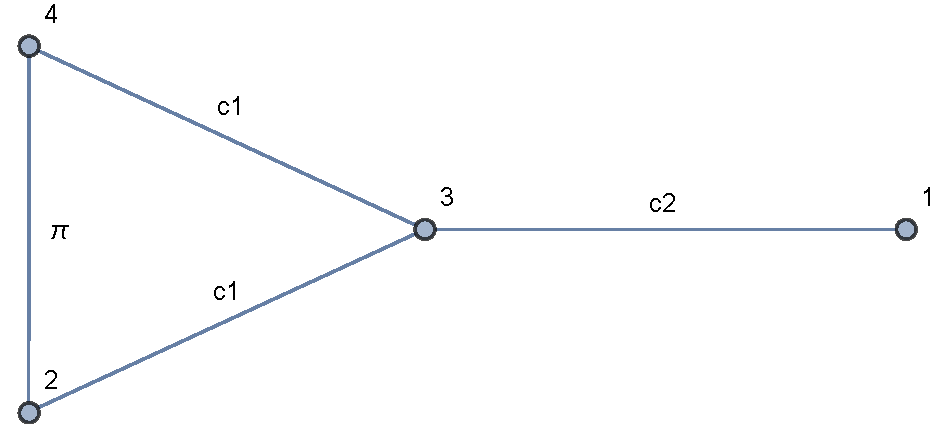
\includegraphics[width=0.7\textwidth]{graph.pdf}
\caption{\label{fig:graph}An example of a metric graph generated by our program. The vertices are labeled by numbers and the edge lengths are indicated. $c1$ and $c2$ are  parameters.}
\end{figure}


\begin{figure}
\centering
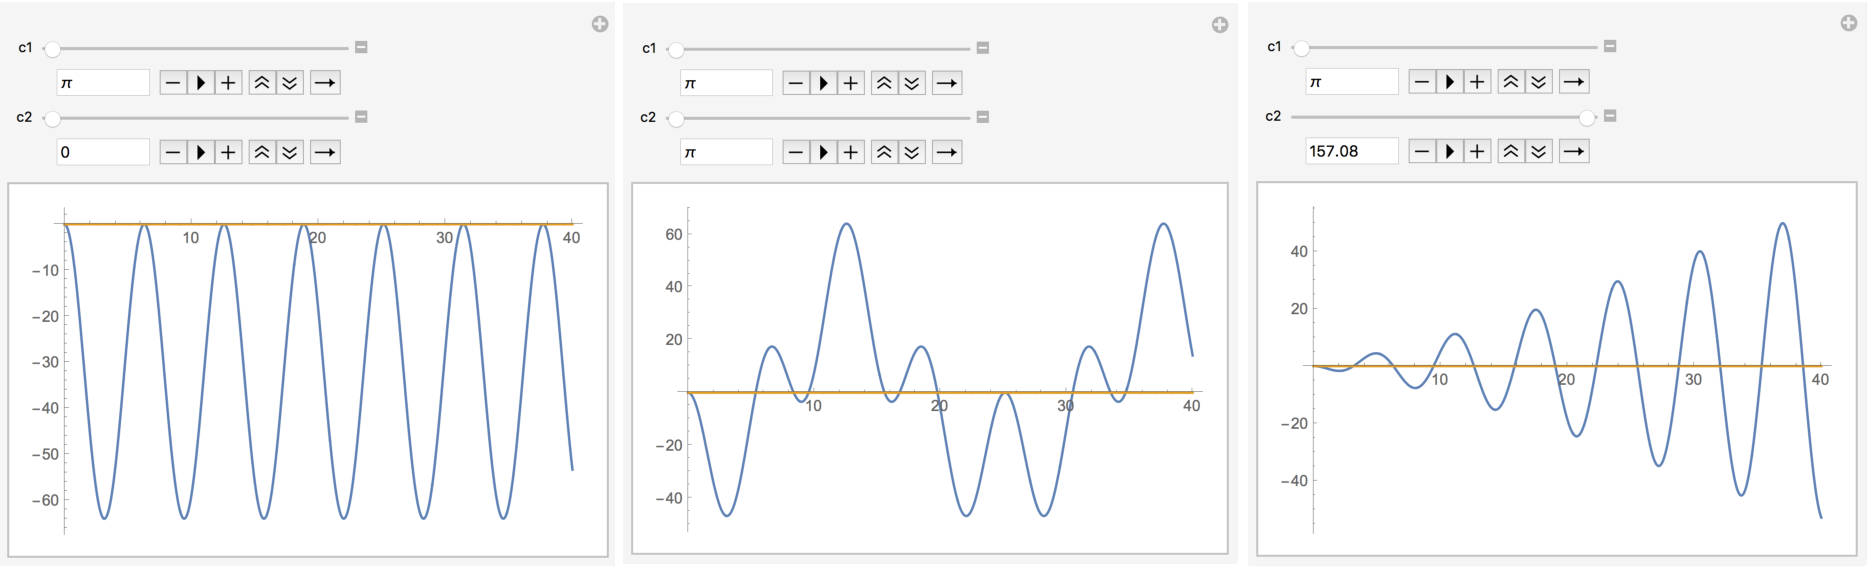
\includegraphics[width=1.0\textwidth]{all.pdf}
\caption{\label{fig:all}Examples of plots of $D(k)$, for the graph shown in Fig. 1, where $c1$ and $c2$ can be changed using sliders. Left panel. Here $c1=\pi$ and $c2=0$ and we have a triangular graph (with length normalized to one). The zeros of $D(k)$ are then at $k=2n\pi$ which is reflected in the figure. Middle panel. Here $c1=c2=\pi$ and it is less obvious where the zeros of $D(k)$ should be located. Right panel. Here $c2=50\pi$ and the graph is almost a path graph, which has zeros of $D(k)$ at $k=n\pi$.}
\end{figure}
\section{Spectral growth of graphs}

\begin{figure}
\centering
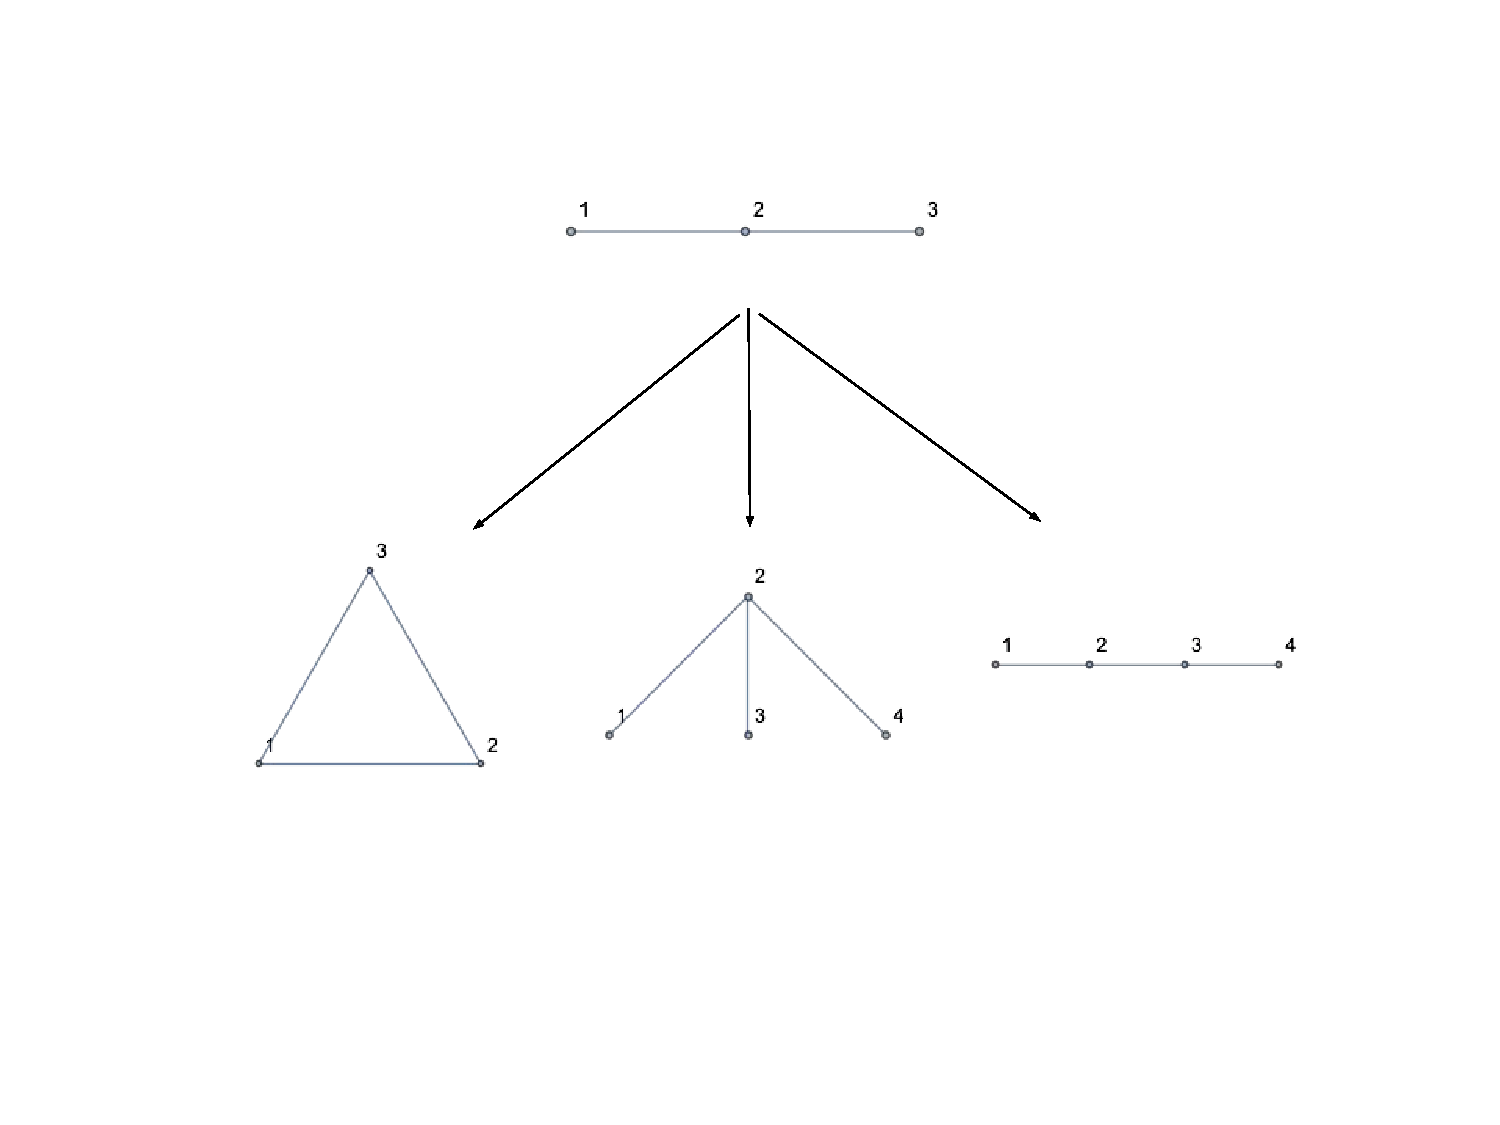
\includegraphics[width=0.5\textwidth]{Parent-child.pdf}
\caption{\label{Parent-child:all}The top graph is the parent graph and has three vertices. From this graph we get three child graphs by adding an edge, shown in the bottom. Out of these child graphs we select the graph which has a spectrum which best fit some chosen criterion. The selected graph becomes a new parent graph and the process is repeated. Note that adding an edge does not necessarily add a vertex.}
\end{figure}

As an application of our program we have grown graphs "spectrally". Most previous studies of graph growths has been of tree growth using local rules \cite{vazquez2003growing}. This is probably motivated by applications. For instance, many growth processes in nature seem to occur by quite local rules, for instance the growth of crystals such as ice crystals and snow flakes. Our growth process is highly non-local. The spectra of quantum graphs are very sensitive to the overall graph structure and cannot be determined by a subgraph of the graph.

The growth or evolution of the graphs proceeds as follows. We define a target goal. This may be a desired spectrum, $\sigma=(\mu_0,\mu_1,\mu_2,...,\mu_N)$ consisting of $N+1$ eigenvalues. $\mu_0$ is always equal to zero since the first eigenvalue of any graph is zero. We then choose a starting parent graph, $\Gamma_1$, most often two edges, each of length 1/2. $\Gamma_1$ will have a spectrum $\sigma(\Gamma_1)$ where we take only the smallest $N+1$ eigenvalues, that is we take an initial segment of the spectrum. We will seldom distinguish between the initial segment of a spectrum and the full spectrum since there cannot be any confusion. We then generate a set of children of $\Gamma_1$ by adding an edge to $\Gamma_1$, as illustrated in Figure 3. In our implementation the length of the added edges is one, meaning that all graphs will be regular graphs. We then normalize the length of the graphs to one. Let us call the new graphs child graphs, $\Gamma_{11}$, $\Gamma_{12}$, $\Gamma_{13}$, ... . They have spectra $\sigma(\Gamma_{11})$, $\sigma(\Gamma_{11})$, $\sigma(\Gamma_{13})$, ... . We then select the child graph which has a spectrum which are closest to the target spectrum,  i. e. we select the child graph $\Gamma_{1i}$ which minimizes $\Vert \sigma(\Gamma_{1i})-\sigma \Vert$, where the norm is the $\ell^2$ norm. $\Gamma_{1i}$ then becomes a new parent graph and we repeat the process until some stopping criterion is satisfied. This  process creates a sequence of graphs, $(\Gamma_{(1)},\Gamma_{(2)},...,\Gamma_{(N)})=(\Gamma_{1},\Gamma_{1i},\Gamma_{1ij},...,\Gamma_{1...k})$.

Many different criteria for choosing child graphs can be used, for instance maximizing $\lambda_1$ (the spectral gap) or maximizing $\lambda_2/\lambda_1$.
The growth of the graphs can also be constrained. We have implemented a version where only trees are grown. Another possibility is to add a graph more complicated than an edge when creating child graphs. It is also possible to delete edges from graphs, which we have implemented. When we delete an edge between two vertices, $v_i$ and $v_j$, we also merge the two vertices into one. Alternating between adding an edge and deleting an edge can create sequences of graphs that have the same size but may change topology as they evolve.



\begin{figure}
\centering
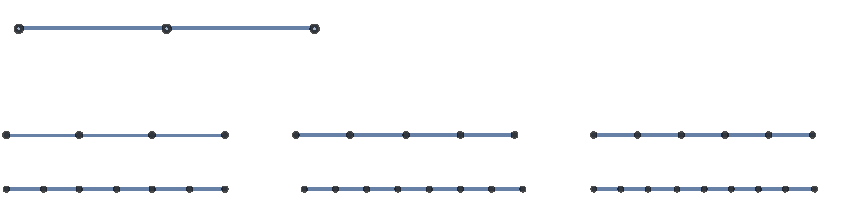
\includegraphics[width=1.0\textwidth]{EdgeGrowth.pdf}
\caption{\label{EdgeGrowth:all}The top graph is the parent graph and has three vertices. From this graph we get the sequence of graphs below. The goal was to have a spectrum with an initial segment which is close to $(0, \pi, 2 \pi)$. This is satisfied by a path graph. The parent graph is simply extended when we evolve the graphs.}
\end{figure}

\begin{figure}
\centering
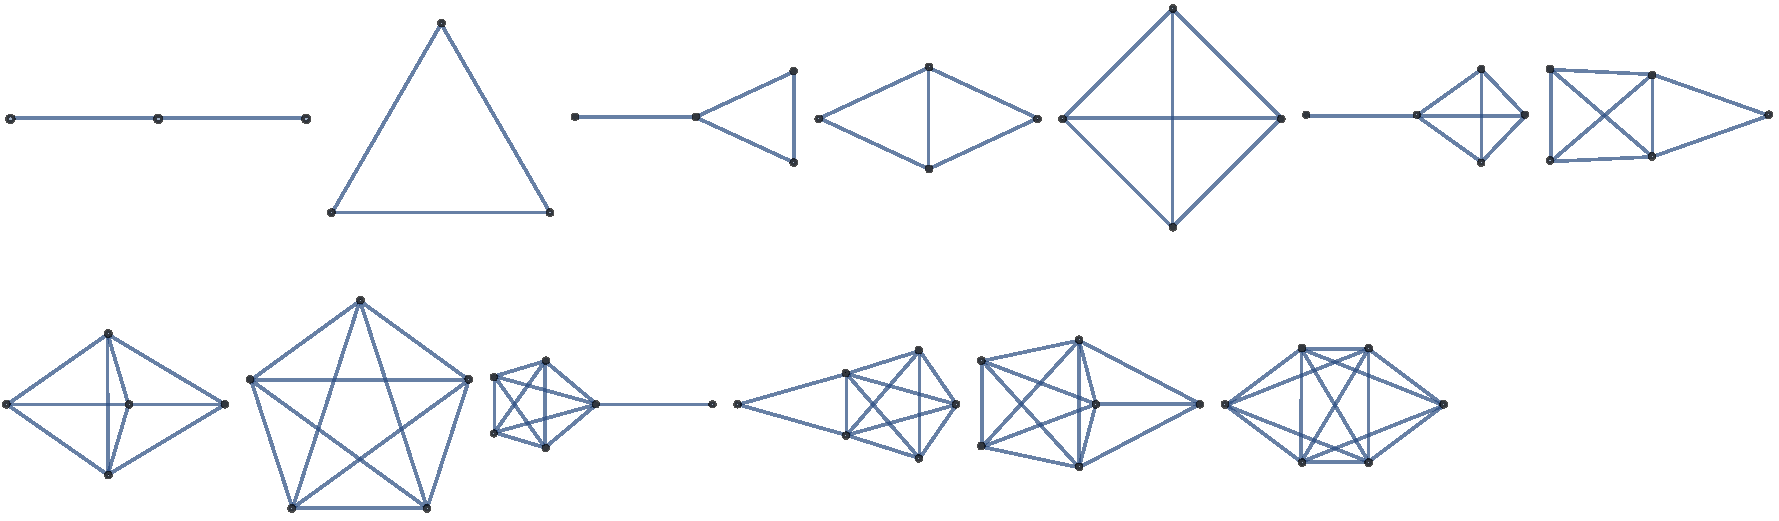
\includegraphics[width=1.0\textwidth]{MaxSpectralGap.pdf}
\caption{\label{MaxSpectralGap:all}In this sequence of graphs the goal was to maximise the spectral gap, $\lambda_{1}$. The graphs are now graphs which contains many complete graphs.}
\end{figure}


\subsection{Experiments}
We will now describe some experiments that we have done. 
\begin{itemize}
  \item In the first experiment, we chose the target spectrum $\sigma=(0, \pi^2, (2\pi)^2)$ and the goal was to minimise $\Vert \sigma(\Gamma_{1i})-\sigma \Vert$. $\sigma$ is the initial part of the spectrum of a path graphs and unsurprisingly the growth of the graphs proceeds by adding an edge to the parent edge graph, simply extending it.
  \item In the second experiment the goal was to maximise $\lambda_{1}$, also known as the spectral gap. We then find that the sequence consists of graphs with a large number of edges compared with vertices and include all complete graphs with equal length edges (equilateral complete graphs). It has been proven that the spectral gap becomes arbitrarily high for equilateral complete graphs when the number of edges increases \cite{kennedy2015spectral}.
  \item In the third experiment the goal was to maximise $\lambda_{2}/\lambda_{1}$. We then find that the sequence consists of graphs (often complete graphsE,<<) which are joined by one edge, also known as dumbbell graphs. From this experiment we conjecture that $\lambda_{2}/\lambda_{1}$ can become arbitrarily large for this class of graphs. We tested this and could reach $\lambda_{2}/\lambda_{1}>64$ before reaching the limit of our laptop computer. In fact testing with dumbbell graphs where two general graphs are joined by one edge we also find that $\lambda_{2}/\lambda_{1}$ can become very large.
  \item In the fourth experiment the goal was to maximise $\lambda_{1}$. The growth was here alternating between adding an edge and deleting an edge. In this case we prefer to use the term evolution rather than growth of the graphs. We started with a grid graph and after a few steps we ended up with a complete graph. After this stage the graphs alternate as illustrated in the figure. If we have the different goal of minimising $\lambda_{1}$ instead of maximising $\lambda_{1}$ the final graph will be a path graph, as expected.
\end{itemize} 
\subsection{Programmed evolution of graphs}
It is also possible to program the growth of the graphs. We made a program with the following pseudocode:
\newline
\newline
\begin{tabbing}
\hspace{0.5cm} \=  \kill
\textbf{Begin}\\ 
\textbf{Initialise} $\Gamma_1$= parent graph, $i=1$\\  
\>  \textbf{Do} $\Gamma_{i+1}$=AddEdge($\Gamma_i$), i=i+1\\ \>\textbf{until} $\lambda_{1}>5\pi$\\
\>  \textbf{Do} $\Gamma_{i+1}$=AddEdgeTree($\Gamma_i$), i=i+1\\
\>  \textbf{until} $\Vert \sigma(\Gamma_{1i+1})-(0,5\pi,15\pi) \Vert \leq 1$\\
  \textbf{Print}($\Gamma_{i+1}$)\\
  \textbf{End}\\
\end{tabbing}  

The command AddEdge adds an edge between two vertices in the parent graph creating a set of child graphs. The command then selects the child graph which is closest to our goal. The command AddEdgeTree adds an edge between the parent graph and a new vertex and then selects the child graph. Both these commands save their selected graphs to memory for later retrieval.

By executing these type of programs one can steer the growth of the graphs to a certain goal such that subgoals are attained on the way. One may also include If-statements in the code and programs of very high complexity can be made, in particular if graphs are stored in memory for later recall and comparisons. Unbounded loops are easily included as can be seen from our pseudocode. One interesting but possibly hard question is to characterise the programs that never terminate. Another interesting question is if it is possible to "help" the graphs to attain a difficult goal by having suitable subgoals to attain first. We have found that some goals are very hard to obtain during our experiments. Unfortunately these types of programming experiments are very taxing for the computer and we could not execute too long programs.

\begin{figure}[h]
\centering
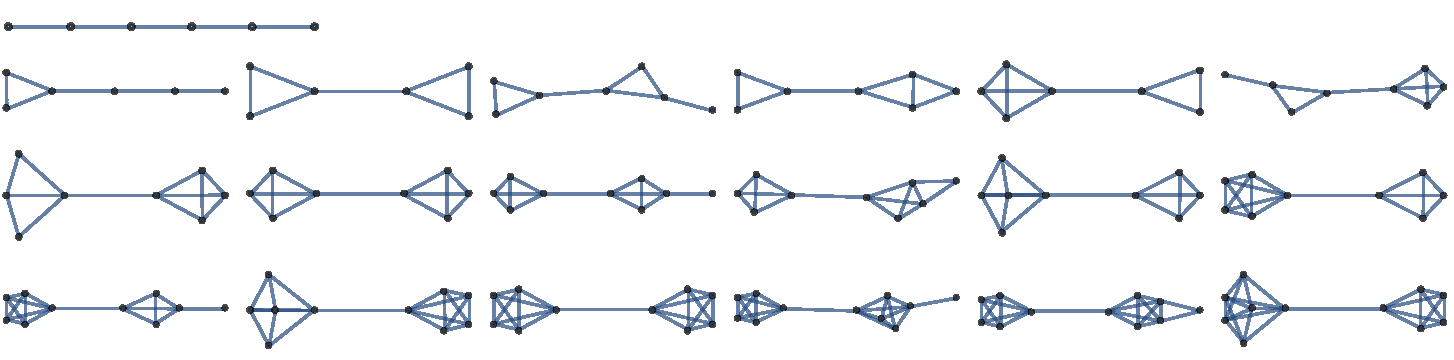
\includegraphics[width=1.0\textwidth]{MaxRatio.pdf}
\caption{\label{MaxRatio:all}In this sequence of graphs the goal was to maximise $\lambda_{2}/\lambda_{1}$. The graphs are two complete graphs joined by one edge. The parent graph is a path graph with six vertices. Not all graphs in the sequence have been plotted.}
\end{figure}

\begin{figure}
\centering
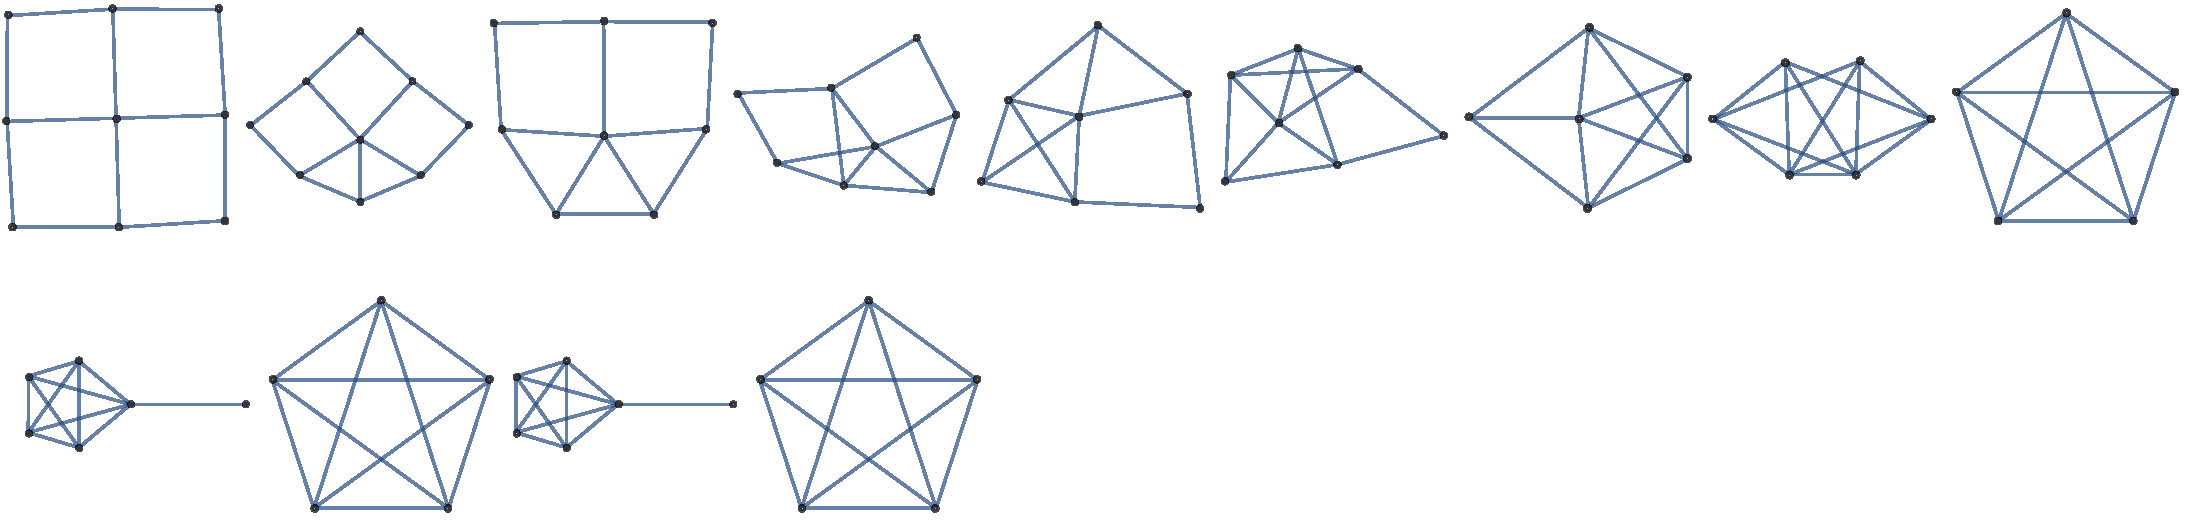
\includegraphics[width=1.0\textwidth]{GridToComplete.pdf}
\caption{\label{GridToComplete:all}In this sequence of graphs we added and then deleted an edge alternatingly, starting with a grid graph. The goal was to maximise the spectral gap, $\lambda_{1}$. The grid graph transforms to a complete graph after eight steps. The sequence then becomes cyclical, alternating between the complete graph and the complete graph with an added edge.}
\end{figure}

\begin{figure}
\centering
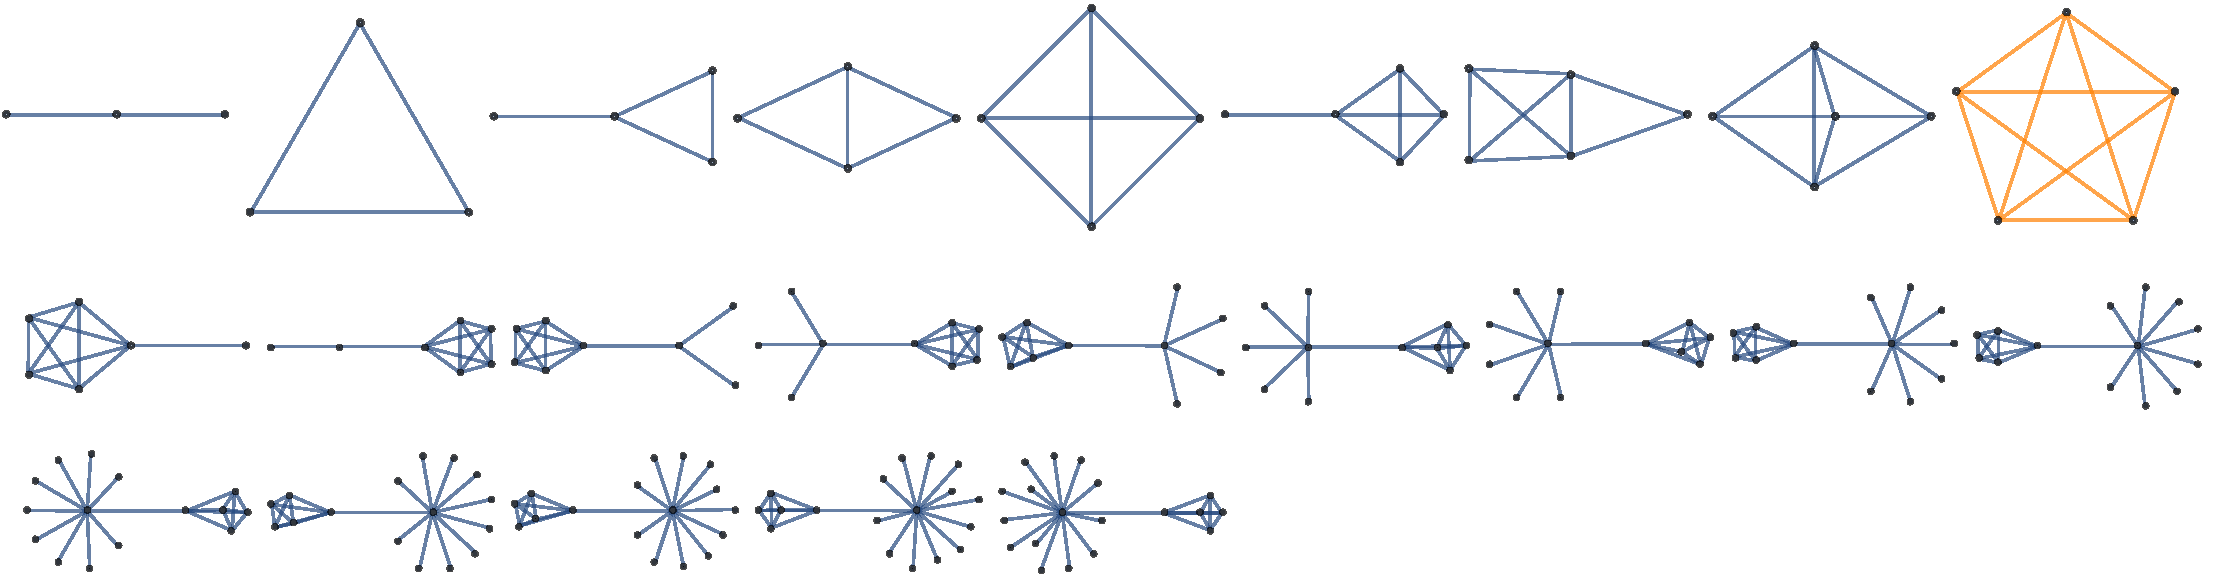
\includegraphics[width=1.0\textwidth]{Program.pdf}
\caption{\label{Program:all}In this sequence of graphs we used a program. The first goal was to increase $\lambda_{1}$ until $\lambda_{1}\geq 5\pi$ by adding an edge. This resulted in a complete graph, yellow in the figure. The goal was then changed to have a spectrum close to $(0, 5\pi,15\pi)$ by adding a vertex and an edge. The growth then proceeded as in the figure.}
\end{figure}

\section{Conclusion and outlook}
We have found that studying the growth of graphs greatly helps our intuition about their spectral properties. One immediately learns that the eigenvalues of the graphs tend to increase with increasing complexity of the graphs. In fact the graph with the smallest $\lambda_1$ is the path graph \cite{nicaise1987spectre}, where $\lambda_1=\pi^2$, which most often is our starting graph. 

We also find that the growth of graphs can help to find patterns that can be made into conjectures and one example was given above, involving the first two non-trivial eigenvalues. Not much is known about the relation between graphs and more than one non-trivial eigenvalue. 
Future work likely will involve finding more conjectures, and possibly also proving them. The fact that our program sometimes can give all solutions in an analytical form is very helpful for such research. Concerning growth of graphs there is a huge number of questions to be answered. Is it for instance possible to have something analogous to phase transitions in the graphs? That is, can a small change in the goal completely change the topology of the graph?

We have released the program that calculates spectra of graphs as open-source under Gnu General Public License \cite{Pistol2016}. The graph growth program is not released yet, since it is not very userfriendly at this stage. 
 
\newpage
\bibliographystyle{unsrt}
\bibliography{bibliography.bib}
\end{document}